\graphicspath{{./images/}}

\chapter{Bausteinsicht}

\section{Beschreibung}

Die Architektur für die Applikation wird mittels vier Schichten realisiert. Die Präsentationsschicht ist auf dem WebServer während die anderen drei sich auf dem AppServer befinden. Die einzelnen Komponenten wurden gruppiert um die Übersicht zu wahren. Auf der nächsttieferen Ebene sind diese Komponenten detailierter aufgeführt.

\newgeometry{left=2.5cm, right=2.5cm, bottom=2.5cm, top=2.5cm}
\begin{landscape}
\section{Ebene 1}

\begin{center}
	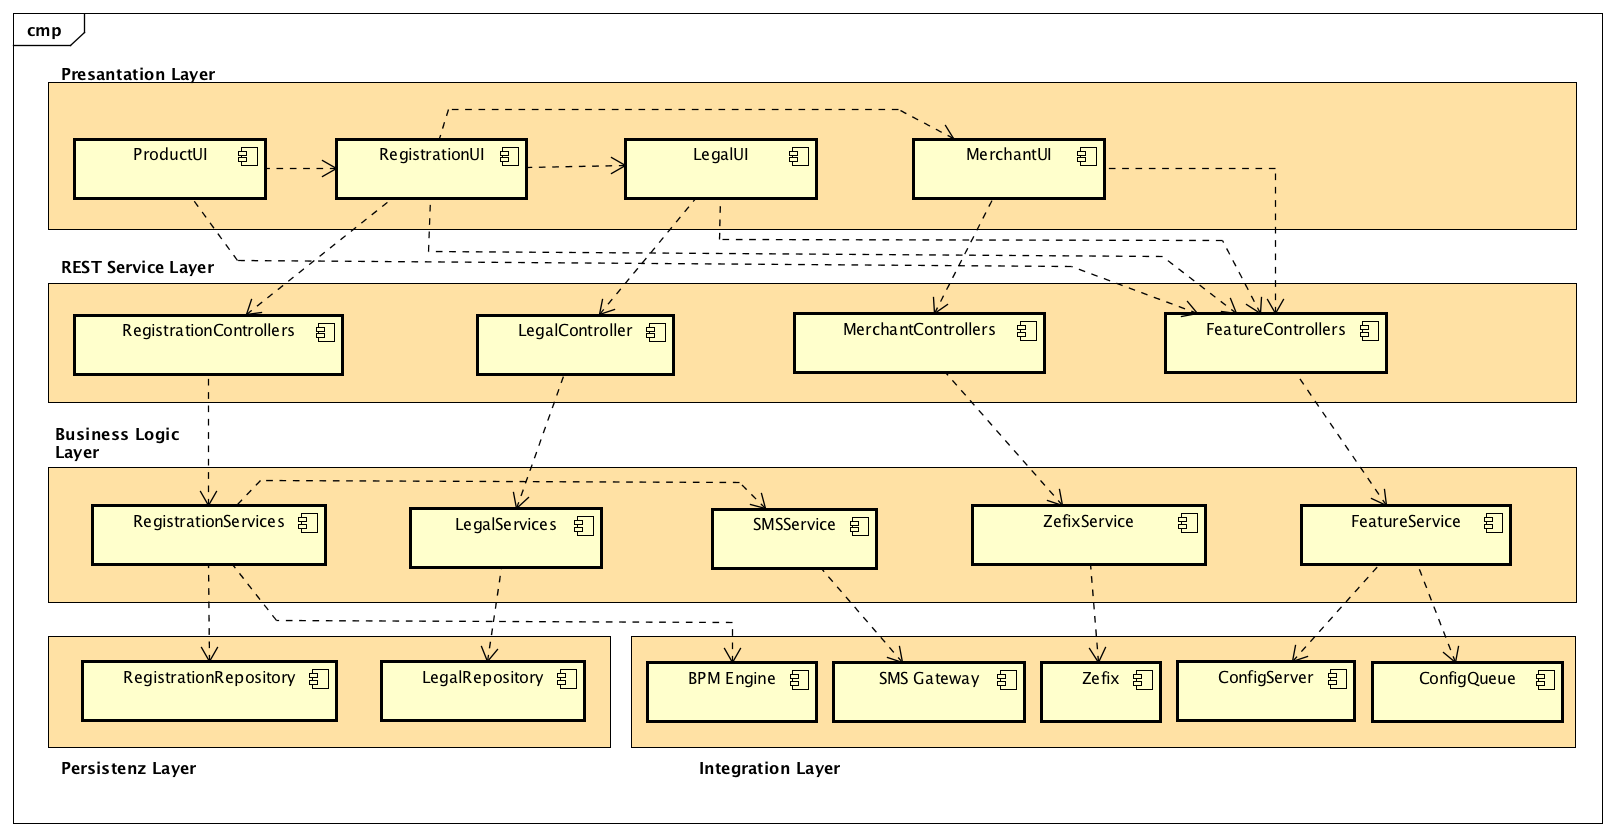
\includegraphics[scale=0.60]{ComponentLevel1.png}
\end{center}

\end{landscape}
\restoregeometry

\begin{table}[H]
	\centering
	\caption{Presentation Layer}
	\begin{tabular}{ | p{4cm} | p{12cm} | }
		\toprule
		{\textbf{Komponente}} & {\textbf{Beschreibung}} \\
		\midrule
		ProductUI &  Stellt die einzelnen Produktoptionen von Twint dar welche der Benutzer auswählen kann. \\ \hline
		RegistrationUI &  Beinhalten sämtliche Felder für die Registration wie Name, Addresse, Händlername. Stellt die Eingabefelder für den Verifikationscode dar welcher dem Benutzer zugesendet wird.\\ \hline
		LegalUI &  Zeigt rechtliche Dokumente wie Allgemeinegeschäftsbedienungen an. \\ \hline
		MerchantUI &  Zuständing für die überprüfung des neuen Händlers.\\
		\bottomrule
	\end{tabular}
\end{table}

\begin{table}[H]
	\centering
	\caption{REST Service Layer}
	\begin{tabular}{ | p{4cm} | p{12cm} | }
		\toprule
		{\textbf{Komponente}} & {\textbf{Beschreibung}} \\
		\midrule
		RegistrationController &  Schnittstelle für den Registrationsprozess und die Verifikation des Codes. \\ \hline
		LegalController &  Schnittstelle welche rechtliche Dokumente liefert. \\ \hline
		MerchantController &  Schnittstelle für die Prüfung von Händlern.\\ \hline
		FeatureController & Schnittstelle für das Abfragen der Features welche aktiv sind. \\
		\bottomrule
	\end{tabular}
\end{table}

\begin{table}[H]
	\centering
	\caption{Business Logic Layer}
	\begin{tabular}{ | p{4cm} | p{12cm} | }
		\toprule
		{\textbf{Komponente}} & {\textbf{Beschreibung}} \\
		\midrule
		RegistrationService &  Enthält sämtliche Logik für die Aufbereitung der Registrierungsanfrage an die Workflow Engine sowie die Überprüfung des SMS Codes welcher an den neuen Händer verschickt wurde.\\ \hline
		LegalService &  Stellt die Dienste für das Abfragen den rechtlichen Dokumente bereit. \\ \hline
		FeatureService &  Verwaltet die aktuell eingeschalteten Features welche aktiviert sind. Holt sich die neuen Konfigurationen automatisch nach einer Benachrichtigung durch die Message Queue. \\ \hline
		SMSService & Ermöglicht das Senden des generieten SMS Codes an den Händler.\\
		\bottomrule
	\end{tabular}
\end{table}

\begin{table}[H]
	\centering
	\caption{Persistenz Layer}
	\begin{tabular}{ | p{4cm} | p{12cm} | }
		\toprule
		{\textbf{Komponente}} & {\textbf{Beschreibung}} \\
		\midrule
		RegistrationRepository &  Speichert die Registrationsdaten den Code sowie die Requests welche nicht direkt zur Workflow Enginge gesendet werden können. \\ \hline
		LegalRepository &  Holt die rechtlichen Dokumente aus dem Datenspeicher. \\
		\bottomrule
	\end{tabular}
\end{table}

\begin{table}[H]
	\centering
	\caption{Integration Layer}
	\begin{tabular}{ | p{4cm} | p{12cm} | }
		\toprule
		{\textbf{Komponente}} & {\textbf{Beschreibung}} \\
		\midrule
		Zefix &  Handelsregisterschnittstelle zu Überprüfung des Händlers \\ \hline
		Configserver &  Beinhaltet die Configurationen der einzelnen Featueres. \\ \hline
		SMS Gateway &  Sendet generierte Code an die vom Händler angegebene Nummer. \\ \hline
		ConfigeQueue & Message Queue welche die Benachrichtigungen für Konfigurationsänderungen enthält. \\ \hline
		BPM Engine & Verarbeitet die Registrierungsdaten im hinterlegten Workflow beschrieben in Kapitel \ref{businesscase}\\
		\bottomrule
	\end{tabular}
\end{table}

\section{Ebene 2}

\section{Ebene 3}